% options:
% thesis=B bachelor's thesis
% thesis=M master's thesis
% czech thesis in Czech language
% slovak thesis in Slovak language
% english thesis in English language
% hidelinks remove colour boxes around hyperlinks

\documentclass[thesis=B,czech]{FITthesis}[2012/06/26]

\usepackage[utf8]{inputenc} % LaTeX source encoded as UTF-8

\usepackage{graphicx} %graphics files inclusion
\graphicspath{ {images/} }

\usepackage{listings}


% \usepackage{amsmath} %advanced maths
% \usepackage{amssymb} %additional math symbols

%\usepackage{indentfirst}

\usepackage{dirtree} %directory tree visualisation

% % list of acronyms
% \usepackage[acronym,nonumberlist,toc,numberedsection=autolabel]{glossaries}
% \iflanguage{czech}{\renewcommand*{\acronymname}{Seznam pou{\v z}it{\' y}ch zkratek}}{}
% \makeglossaries

\newcommand{\tg}{\mathop{\mathrm{tg}}} %cesky tangens
\newcommand{\cotg}{\mathop{\mathrm{cotg}}} %cesky cotangens

% % % % % % % % % % % % % % % % % % % % % % % % % % % % % %
% ODTUD DAL VSE ZMENTE
% % % % % % % % % % % % % % % % % % % % % % % % % % % % % %

\department{Katedra počítačových systémů}
\title{Nástroj pro správu a monitorování systému souborů ZettaByte}
\authorGN{Tomáš} %(křestní) jméno (jména) autora
\authorFN{Šimáček} %příjmení autora
\authorWithDegrees{Tomáš Šimáček} %jméno autora včetně současných akademických titulů
\supervisor{Ing. Zdeněk Muzikář, CSc.}
\acknowledgements{Doplňte, máte-li komu a za co děkovat. V~opačném případě úplně odstraňte tento příkaz.}
\abstractCS{Tato práce práce se zabývá problematikou administrace souborového systému ZFS na operačním systému Solaris. Její součástí je popis základních struktur, principů a administračních technik ZFS.
Praktická část práce je věnována návrhu a popisu implementace administrátorského nástroje, který slouží pro monitorování a správu souborového systému ZFS v operačním systému Solaris. Návrh klade důraz především na bezpečnost a budoucí rozšiřitelnost výsledného nástroje. }
\abstractEN{This thesis deals with issues of administrating Zettabyte file system on operating system Solaris. It describes basic structure, internal principles and administrating techniques of ZFS. The practical part deals with design and implementation of administrating tool that will serve for monitoring and managing ZFS. The design is focused mainly on security, extensibility and integration to operation system Solaris. }
\placeForDeclarationOfAuthenticity{V~Praze}
\declarationOfAuthenticityOption{4} %volba Prohlášení (číslo 1-6)
\keywordsCS{Souborový systém Zettabyte, Solaris, webové rozhraní, administrace, monitorování \clearpage }
\keywordsEN{Zettabyte file system, Solaris, web interface, administration, monitoring}

\begin{document}

% \newacronym{CVUT}{{\v C}VUT}{{\v C}esk{\' e} vysok{\' e} u{\v c}en{\' i} technick{\' e} v Praze}
% \newacronym{FIT}{FIT}{Fakulta informa{\v c}n{\' i}ch technologi{\' i}}

\begin{introduction}
    Tato práce se věnuje administraci souborového sytému Zettabyte. Popisuje návrh a implementaci grafického nástroje pro jeho monitorování a správu.

Souborový systém Zettabyte (ZFS) je jeden z mnoha souborových systémů, se kterými se dnes můžeme setkat.
Byl vyvinut společností Sun Microsystems a integrován do operačního systému Solaris. Tento souborový systém dokáže spravovat velké množství dat díky své 128-bitové architektuře a mimo jiné nabízí funkce pro ověřování integrity dat, správu fyzických úložišť, vlastní softwarový RAID a v neposlední
řadě také šifrování dat. Jedním z nedostatků tohoto souborového systému je absence grafického rozhraní pro jeho správu. ZFS nabízí administrátorovi pouze rozhraní na příkazové řádce.

Hlavním cílem této bakalářské práce je navrhnout a implementovat graficky orientovanou nadstavbu souborového systému ZFS, která bude umožňovat jeho monitorování a správu. Tento nástroj bude koncentrovat funkcionalitu ZFS do jednoho místa, aby usnadnil uživateli správu tohoto souborového sytému.

Struktura této bakalářské práce se skládá ze šesti hlavních kapitol.
V první kapitole je objasněn důvod, proč by měl být tento administrátorský nástroj vytvořen a jaký přínos by jeho implementace měla pro různé skupiny uživatelů souborového systému ZFS.
Druhá kapitola popisuje účel souborových systémů a představuje jejich nejznámější zástupce. V závěrečné části této kapitoly je uvedeno krátké porovnání základních parametrů vybraných souborových systémů.
V úvodu třetí kapitoly je stručně představen souborový systém ZFS, jeho historie a vnitřní struktury. Hlavním obsahem této kapitoly je představení základních administračních funkcí a zajímavých principů, které může administrátor využívat.
Čtvrtá kapitola rozebírá několik vybraných nástrojů, které slouží pro monitorování nebo administraci ZFS. Hlavním účelem analýzy těchto nástrojů je objevení jejich kladných a záporných stránek. Implementace výsledného nástroje by se mohla opírat o tyto poznatky a naopak by se mohla vyvarovat případným chybám a problémům, které vybrané nástroje obsahují.
Úvod páté kapitoly definuje požadavky, které bude implementovaný nástroj splňovat. Hlavní obsah této kapitoly se týká návrhu architektury, volby uživatelského rozhraní a analýzy bezpečnostních rizik administrátorského nástroje.
Téma poslední šesté kapitoly je samotná implementace navrhnutého nástroje. V této kapitole jsou představeny a stručně popsány jednotlivé komponenty aplikace. Pozornost je také věnována integraci nástroje do operačního systému Solaris a implementaci bezpečnostních opatření, které budou sloužit pro bezpečný chod aplikace.
Po hlavních kapitolách následuje stručný závěr, kde je shrnuto, zda bylo dosaženo stanovených cílů a také jsou zde uvedeny některé možnosti budoucího rozšíření implementovaného nástroje.

Nezbytnou součástí této práce jsou zdrojové kódy aplikace a uživatelská příručka, která popisuje instalaci, konfiguraci a spuštění nástroje. Aplikace i příručka jsou dostupné na přiloženém médiu.




\end{introduction}

\chapter{Cíle práce}
    V této kapitole je přiblížena problematika, kterou se tato bakalářská práce zabývá. V závěru jsou zmíněny výhody, které by případné vyřešení problematiky mohlo přinést.

\section{Problematika}
Následující problém si můžeme zobecnint na většinu nástrojů či aplikací, které slouží k administraci nějakého systému. U rozsáhlých systémů platí, že s rostoucím počtem funkcí, které systém nabízí, roste i složitost jeho administrace. Aby administrátor mohl rychle a efektivně spravovat tyto systémy, musí důkladně znát všechny jejich funkce a principy. V případě ZFS se jedná o desítky příkazů, které slouží pro ovládání souborového systému. I proto společnost Oracle vydává mnoho online návodů, které společně s manuálovými stránkami jednotlivých příkazů vytvářejí dobrý zdroj informací pro administrátory ZFS.



Pro zkušené administrátory, kteří se v prostředí tohoto souborového systému pohybují jíž delší dobu, je příkazová řádka pravděpodobně nejrychlejší a nejefektivnější volbou. Potřebný příkaz stačí napsat do příkazové řádky a sytém ho provede. Administrátor může tyto příkazy použít ve skriptech, které může využít pro automatizaci některých činností. Na druhou stranu existují uživatelé, kteří se teprve seznamují se souborovým systémem ZFS a nemají potřebné znalosti. Jelikož v ZFS neexistuje grafické rozhraní, kde by byla funkcionalita sdružena na jednom místě, musí začínající uživatelé často využívat návodů nebo manuálových stránek.
\section{Řešení}
Z výše uvedených důvodů jsem se rozhodl navrhnout a implementovat graficky orientovaný administrátorský nástroj pro ZFS, který by sdružoval funkcionalitu ZFS do jednoho místa. Z tohoto místa by administrátor mohl pohodlně ovládat funkce systému. Tento nástroj by měl být určený především pro seznámení uživatelů se souborovým systémem ZFS a jeho základními funkcemi.


\chapter{Souborové systémy}
    V~úvodu této kapitoly je uvedena definice souborového systému, která je následována výčtem nejznámějších zástupců souborových systémů. V~závěru této kapitoly porovnáme několik vlastností vybraných souborových systémů.
\section{Souborový systém}
    \label{fs}
    Souborový systém označuje způsob, kterým se organizují data v~datových úložištích. Jak už název napovídá, data jsou v~úložišti organizována do souborů. Soubory umožňují ukládání informací na disku a adresáře tyto informace umožňují hierarchicky uspořádat \cite{fs}. Tento systém si o~každém souboru udržuje informace, aby bylo později možné zjistit, kde se soubor nachází nebo jak je velký. Dále tento systém umožňuje tyto data číst, měnit nebo vytvářet.

    V~dnešní době existuje mnoho způsobů organizace dat, a proto máme k~dispozici i mnoho různých souborových systémů. Ty se liší nejenom ve způsobu organizace dat,
    ale také ve velikosti datového úložiště, které dokáží adresovat. Dalším rozlišovacím prvkem může být závislost na operačním systému.
    Jelikož nejrozšířenější operační systémy jsou systémy typu UNIX a Windows, uvedeme několik typických zástupců souborových systémů pro tyto platformy.

    Mezi nejznámější zástupce UNIXových souborových systémů patří následující systémy:
    \begin{itemize}
      \item UFS
      \item ext2, ext3, ext4
    \end{itemize}

    Mezi nejznámější zástupce souborových systémů pro platformu Windows se řadí následující systémy:
    \begin{itemize}
      \item FAT12, FAT16, FAT32
      \item NTFS
    \end{itemize}

\section{Porovnání}
    V~tabulce \ref{fscompare} můžeme vidět porovnání vybraných souborových systémů z~hlediska velikosti diskové adresy, velikosti datových bloků a maximální velikosti svazku, který dokáží spravovat.
    \begin{table}
    \centering
    \caption{Porovnání souborových systémů \cite{fs}}
    \label{fscompare}
    \begin{tabular}{|c|c|c|c|}
    \hline
    Název & Velikost adresy & Velikost bloku & Max. velikost svazku \\ \hline
    FAT-32 & 28b & 4KB-32KB & 2TB \\ \hline
    NTFS & 64b & 512B-64KB & 16EB \\ \hline
    ZFS & 128b & 512B-128KB & 256ZB \\ \hline
    \end{tabular}
    \end{table} 

\chapter{ZFS}
    \input{chapters/zfs.tex}

\chapter{Analýza implementovaných řešení}
    V následující kapitole je rozebráno několik nástrojů sloužící pro monitorování a správu souborového systému ZFS. Hlavně ním předmětem analýzy jsou výhody a nevýhody implementovaných řešení. Výhody těchto nástrojů by mohly pomoci ke správnému návrhu vlastního řešení administračního nástroje pro ZFS.
\section{zfsmon}
V analýze implementovaných řešení je kladen důraz především na nástroj \emph{zfsmon}. Tento nástroj slouží pro monitorování souborových systémů ZFS na více oddělených souborových serverech. Aplikace se dá rozdělit na dvě hlavní části, které spolu spolupracují.

První částí je skript, který běží na počítači se souborovým systémem ZFS. Tento skript je spouštěn pomocí \emph{crontabu} a zajišťuje aktualizaci informací v databázi, která je součástí webové aplikace. V unixových operační systémech \emph{crontab} zajišťuje automatické spouštění programů v určitých intervalech. Doporučený interval spouštění skriptu nástroje \emph{zfsmon} je 15 minut \cite{zfsmon}.

Druhou částí aplikace \emph{zfsmon} je samotná webová aplikace, která se stará o zobrazování dat z databáze. V databázi se nacházejí informace o stavu jednotlivých souborových systémů z různých serverů. Aplikace zobrazuje tyto informace klientovi v podobě HTML stránek.

Velkou výhodou této aplikace je, že dokáže zobrazovat informace z více oddělených úložišť najednou. Na druhou stranu způsob zpracování dat přináší značnou nevýhodu, která spočívá v intervalu aktualizace dat v databázi. V průběhu tohoto intervalu aplikace znemožňuje uživateli vidět aktuální data ze souborového serveru. Uživatel je nucen počkat na konec tohoto intervalu, kdy jsou opět nahrána aktuální data do databáze. Další nevýhodou tohoto nástroje je absence veškeré funkcionality, která by se týkala administrace souborového systému ZFS.

Tento nástroj nám tedy umožňuje kvalitně monitorovat informace z více zdrojů najednou, ale neposkytuje nám možnost jakékoli administrace monitorovaných souborových systémů.
\section{zfswatcher}
Druhým nástrojem, který slouží pro monitorování souborového systému ZFS, je nástroj jménem \emph{zfswatcher}.

Tento nástroj slouží jako webové rozhraní pro sledování souborového systému ZFS. Stejně jako předchozí nástroj zpracovává periodicky data a zobrazuje je pomocí HTML stránek, s čímž souvisí stejný problém, který se vyskytuje u předhozího nástroje. Oproti nástroji \emph{zfsmon} umí zobrazovat informace pouze z jednoho souborového serveru. Na druhou stranu tento nástroj umí, v případě změny stavu ZFS, poslat upozornění v podobě e-mailu nebo zalogování do logu \cite{zfswatcher}.
\section{ZFS administration console}
Na závěr této kapitoly zmíníme ještě nástroj \emph{smcwebserver}. Tento nástroj je součástí operačního systému Solaris 10 6/06 a umožňuje administrátorovi spravovat některé funkce tohoto operačního systému. Mimo jiné se část tohoto nástroje věnuje právě správě souborového systému ZFS \cite{smc}. Bohužel v novější verzi Solarisu 11 se tento nástroj již nevyskytuje. Jako jediný ze zmíněných nástrojů právě \emph{smcwebserver} nabízí administrátorovi funkce pro správu souborového systému ZFS.

\chapter{Návrh řešení}
    Následující kapitola popisuje návrh nástroje pro administraci souborového systému ZFS. Zaměřuje se především na architekturu a bezpečnostní opatření navrhované aplikace.
\section{Požadavky}
Na začátku bychom měli stanovit funkcionalitu, která bude od aplikace vyžadována. Ještě jednou si připomeneme, že hlavním cílem této práce je vytvořit graficky orientovaný administrační nástroj pro správu souborového systému ZFS.

Souborový systém ZFS byl původně integrován do operačního systému Solaris. I přes to, že dnes již existují operační systémy, na které bylo ZFS přeneseno, hlavní platformou aplikace bude právě operační systém Solaris.

Jelikož má nástroj být grafického charakteru, můžeme brát jako první požadavek na aplikaci přítomnost uživatelského rozhraní.

Jak bylo zmíněno v úvodu, účelem toho nástroje má být ulehčení a zpřehlednění správy souborového systému ZFS a to i pro začínajícího administrátora. Bylo by tedy vhodné, aby zvolené uživatelské rozhraní bylo přehledné a jednoduché na používání.

ZFS je souborový systém určený především pro servery. Tyto počítače mohou být v mnohých situací pro administrátora fyzicky nedostupné. Abychom umožnili administrátorovi správu i v těchto situací, bude náš nástroj poskytovat možnost vzdáleného přístupu ke správě ZFS.

Na konci předchozí kapitoly jsme se dozvěděli, že většina nástrojů využívá takový způsob sběru dat, který uživateli v některých situací znemožňuje vidět přímo aktuální data. Tohoto problému bychom se při návrhu měli vyvarovat a zvolit takový způsob, který by uživateli zobrazil aktuální data při každém jeho požadavku.

Další nedostatek objevený při analýze již vytvořených nástrojů pro správu ZFS, je ten, že většina těchto nástrojů vůbec neposkytuje funkce pro administraci. Dovolují nám tedy daný souborový systém sledovat, ale ne ho spravovat. Jelikož je ZFS rozsáhlý souborový systém, obsahuje i velké množství funkcí a příkazů pro jeho správu. Bylo by tedy dobré některé základní funkce a příkazy pro administraci ZFS do tohoto nástroje zahrnout.

Posledním bodem požadavků by měla být bezpečnost. Hlavním důvodem proč se starat o bezpečnost apliakace je fakt, že pomocí ZFS lze jednoduchým příkazem zničit vše co se na disku nachází. Jelikož se z disku načítá při startu i operační systém, mohly by následky být fatální. Příklad, jak se před tímto problémem chránit, si můžeme vzít z UNIXových operačních systémů. Na těchto systémech existuje uživatel \emph{root}, který v systému může dělat všechny operace. Druhou skupinou jsou obyčejní uživatelé, kteří nebezpečné příkazy vykonávat nemohou. To nás může přivést na myšlenku, že aplikace bude přístupná pouze specifikovaným uživatelům.

Pro shrnutí můžeme požadavky na administrační nástroj shrnout do následujících bodů.
\begin{itemize}
    \item Solaris
    \item Uživatelské rozhraní
    \item Jednoduchost a přehlednost
    \item Vzdálený přístup
    \item Aktuálnost dat
    \item Základní funkce pro administraci
    \item Bezpečnost
\end{itemize}

Pokud splníme všechny stanovené požadavky, můžeme uživateli zajistit bezpečnou správu souborového systému ZFS, která mu bude poskytovat aktuální informace.
\section{Možnosti uživatelských rozhraní}
Pro návrh uživatelského rozhraní aplikace přicházejí v úvahu následující možnosti.
    \subsection{Příkazová řádka}
    Každý uživatel, který se někdy nějakým způsobem setkal s administrací UNIXových operačních systémů, by měl mít alespoň nějaké povědomí o tom, co je to příkazová řádka. Příkazová řádka je v UNIXu nástroj, který umožňuje využívat různé příkazy. Je rychlý, nenáročný a jediné co potřebujete vědět je, jaký příkaz napsat a co daný příkaz udělá. Vše se obejde bez myši a klikání.

    Na druhou stranu může být pro začínajícího uživatele složité si všechny příkazy pamatovat a nějakou dobu trvá, než získá potřebné zkušenosti s tímto nástrojem. Pokud uživatel příkazy příliš neovládá, je to pro něj spíše zpomalení práce než zrychlení.

    Protože jsme si v požadavcích stanovili, že náš nástroj má být jednoduchý, přehledný a uživatelsky příjemný na používání i pro začínající uživatele, je tato volba nevhodná.
    \subsection{Grafické rozhraní}
    Jelikož jsme zavrhli příkazovou řádku, je třeba přijít s něčím, co bude pro uživatele přívětivé. Každý uživatel počítače se již jistě setkal s pojmem grafické rozhraní. Pokud ne, pod pojmem grafické rozhraní si můžeme představit například kalkulačku z operačního systému Windows. Prakticky všechno v operačním systému Windows má svoje grafické rozhraní, aby měl uživatel přehled o tom, co může v daný okamžik využívat za funkce.

    Grafické rozhraní nám pomůže vyřešit problém s uživatelským komfortem. Dále nám podle požadavků zbývá zvážit možnost vzdáleného přístupu. Ano i v tomto případě bychom byli schopni tento požadavek splnit. Jde o to, jak by to pro nás bylo pohodlné. Aplikaci by musela být nainstalovaná na každém počítači, ze kterého bychom chtěli ZFS administrovat. Tento problém není nepřekonatelný, ale existuje ještě jedno komfortnější a dnes stále populárnější řešení.
    \subsection{Webové rozhraní}
    Tímto řešením je použití webového rozhraní. Hlavní výhodou toho řešení je fakt, že pro přístup k aplikaci potřebujeme jen webový prohlížeč. Ten je dnes přítomný v drtivé většině operačních systémů. Tato skutečnost nám přináší možnost přistupovat k aplikaci z webového prohlížeče v libovolném operačním systému, přestože aplikace poběží na operačním systému Solaris.

    Webové stránky jsou navíc známé pro většinu uživatelů a tak by při správném návrhu stránek neměl být sebemenší problém s jednoduchostí a přehledností tohoto nástroje.

    Zbytek požadavků jako je bezpečnost jednoduše splníme pomocí správné implementace tohoto řešení.
\section{Architektura aplikace}
V předchozí kapitole jsme pro náš nástroj zvolili možnost zobrazování dat pomocí webového rozhraní. Toto rozhraní se bude skládat z webových stránek, které budeme chtít uživateli zobrazovat. Pro tento účel si budeme muset zvolit nebo implementovat nějaký webový server, který bude zprostředkovávát komunikaci mezi naší aplikací a klientským prohlížečem. Jakmile uživatel požádá pomocí svého prohlížeče o nějakou stránku, server tento požadavek obdrží a předá ho naší aplikaci. Aplikace ho vyhodnotí a prostřednictvím webového serveru pošle uživateli odpovídající odpověď.

Náš nástroj má sloužit pro správu souborového systému ZFS a tak bude nutné vymyslet, jak bude naše aplikace s tímto systémem komunikovat. Administrátor může ZFS spravovat pomocí příkazů, které jednoduše zadá do příkazové řádky. Tyto příkazy dokáží změnit vnitřní stav souborového systému nebo vyvolat nějakou akci. Bude tedy nutné vymyslet vrstvu aplikace, která bude tyto příkazy sestavovat a následně provádět. Na obrázku \ref{architecture} můžeme vidět graficky znázorněnou komunikaci mezi hlavními komponenty aplikace.
\begin{figure}[h]
        \caption{Struktura aplikace}
        \label{architecture}
        \centering
        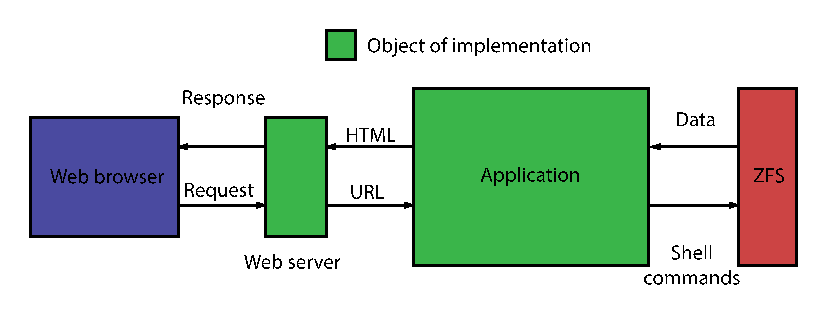
\includegraphics[scale=0.8]{appstructure.pdf}
\end{figure}
    \subsection{Architektura MVC}
    Nyní navrhneme řešení, jak bude aplikace fungovat uvnitř. Jak již bylo zmíněno, náš nástroj bude umožňovat správu souborového systému ZFS pomocí jeho základních funkcí. Tudíž ne všechny funkce budou ve výsledné implementaci zahrnuty. Z tohoto důvodu je aplikaci nutno navrhnout tak, aby se dala jednoduše rozšiřovat o potřebnou funkcionalitu.

    K tomuto účelu použijeme objektový návrh společně s architekturou MVC. Model-view-controller (MVC) je softwarová architektura, která rozděluje aplikaci do tří vrstev tak, že jsou na sobě minimálně závislé \cite{mvc}. Pokud bychom chtěli naši aplikaci rozšířit o novou fukncionalitu, jednoduše stačí rozšířit požadovanou vrstvu.

    Komponenty jednotlivých vrstev aplikace rozdělujeme na \emph{model}, \emph{view} a \emph{controller}.

        \subsubsection{Datová vrstva}
        \verb|Model| je označení pro třídu, která je součástí datové vrstvy aplikace. Úkol této třídy, potažmo i celé datové vrstvy, je manipulace a práce s daty. Jako příklad si můžeme vzít třídu, která má na starost práci s databází. Tato třída obdrží od vyšší vrstvy data a je požádána aby s nimi provedla určitou akci. V databázi může například vytvořit nový záznam popřípadě nějaký modifikovat. V našem případě žádnou databázi potřebovat nebudeme. Všechny datové struktury si ZFS spravuje samo a my k nim nemáme přímý přístup. Naše datová vrstva a její třídy nám tedy budou zajišťovat vykonávání ZFS příkazů, které budou sestaveny na základě dat předaných z logické vrstvy.
        \subsubsection{Prezentační vrstva}
        Další vrstvou aplikace je tzv. prezentační vrstva. Tato vrstva se skládá z tříd nesoucí obecný název \verb|View|. Hlavním úkolem této vrstvy je vykreslování dat uživateli. V grafických aplikacích jsou jednotlivé třídy přímo zodpovědné za vykreslování určitých částí výsledného uživatelského rozhraní. V našem případě aplikace poběží na počítači se souborovým systémem ZFS a uživatel se k ní bude připojovat pomocí webového prohlížeče. Naše prezentační vrstva nebude přímo vykreslovat uživatelské rozhraní, protože neví kam. Pro zachování nezávislosti jednotlivých vrstev, bude prezentační vrstva pouze generovat HTML kód stránky z dat, které jí budou předány. Následně takto vygenerovanou stránku předá zpět do logické vrstvy, která zařídí odeslání stránky uživateli.
        \subsubsection{Logická vrstva}
        Poslední vrstvou aplikace je logická vrstva. Hlavním úkolem této vrstvy je řízení toku dat mezi datovou a prezentační vrstvou. V okamžiku, kdy webový server obdrží nějaký požadavek od uživatele, aplikace vybere z logické vrstvy třídu, která dokáže tento požadavek vyřídit. Tato třída, kterou obecně nazýváme \verb|Controller|, může požádat datovou vrstvu, aby provedla potřebné operace se souborovým systémem nebo od souborového systému získala potřebná data. Následně data převede do potřebného formátu a požádá prezentační vrstvu o jejich vykreslení. V našem případě vykreslená data opět převezme a předá aplikaci, aby je mohla odeslat klientovi.

        Komunikace mezi jednotlivými vrstvami aplikace je znázorněna na obrázku \ref{mvc}. Na obrázku je také vidět způsob předávání dat mezi webovým serverem a aplikací.

    \begin{figure}[h]
        \caption{Architektura aplikace}
        \label{mvc}
        \centering
        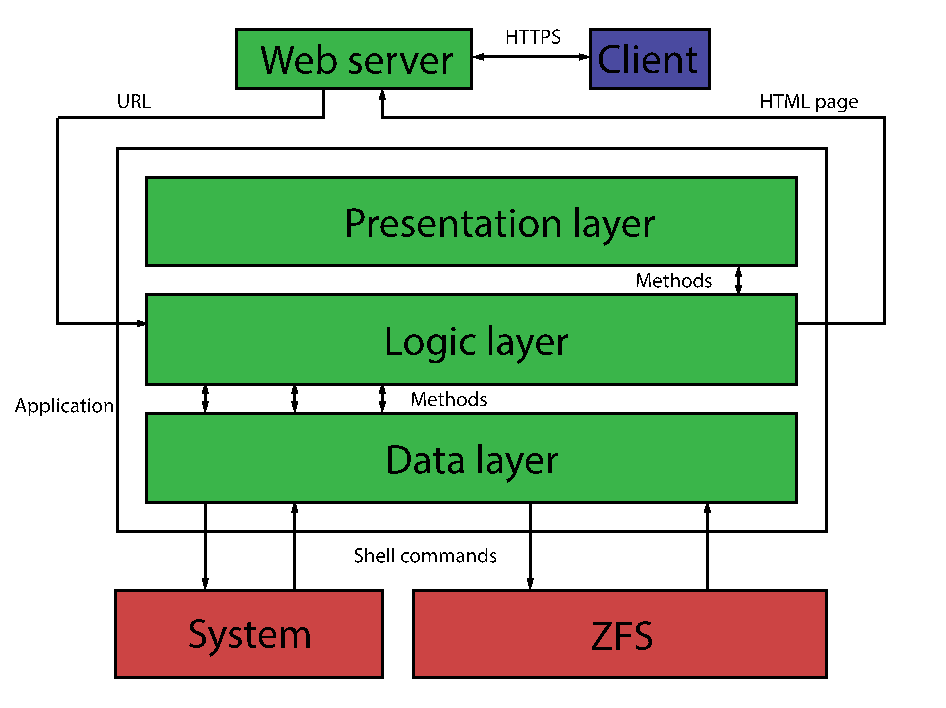
\includegraphics[scale=0.8]{mvc.pdf}
    \end{figure}
\section{Interakce s aplikací}
K aplikaci bude administrátor moci přistupovat pomocí webového prohlížeče. Tato výhoda pramení ze způsobu přenosu webových stránek pomocí protokolu HTTP, který je pro tento účel určený. Jeho definici můžeme najít v RFC dokumentu \cite{RFC2616}. V dnešní době je to jeden z nejpoužívanější protokolů a to zejména proto, že se používá i v internetu. Tento protokol je postavený na architektuře klient-server, kdy klient posílá požadavky na webový server a ten klientovi odpovídá v podobě HTML dokumentu. Jak již bylo zmíněno, výhodou tohoto způsobu je oddělenost serveru a klienta. Webový prohlížeč může uživatel klidně spouštět na operačním systému Windows nebo Linux, zatímco celá aplikace s webovým serverem bude spouštěna pod operačním systémem Solaris.

Uživatel bude pomocí webového prohlížeče vznášet požadavky na webový server v podobě URL. Uniform resource locator (URL) se používá pro lokalizování zdrojů na internetu poskytnutím jedinečného řetězce znaků \cite{RFC3986}. HTTP požadavek, který uživatel bude pomocí webového prohlížeče odesílat, obsahuje právě tento URL řetězec. Tím administrátor specifikuje jakou stránku chce zobrazit popřípadě jakou akci chce povést.

Naši aplikaci tedy postavíme tak, aby byla schopná přijmout URL řetězec a na základě jeho struktury provedla určitou akci.

\section{Bezpečnost}
Další důležitou kapitolou v procesu návrhu administrátorského nástroje je bezpečnost.

Některé příkazy poskytované souborovým systém ZFS jsou dostupné každému uživateli v systému. Jedná se hlavně o příkazy, které vypisují nejrůznější informace o stavu souborových systémů a poolů. Prováděním těchto příkazů se v nastavení ZFS nic nezmění, a proto nemůže dojít k poškození nebo ztrátě dat. Na druhou stranu ZFS nabízí příkazy, které běžní uživatelé nemohou využívat. K provádění těchto příkazů je potřeba oprávnění \emph{root} uživatele. Jedná se zejména o příkazy, které vytvářejí, mění nebo ničí souborové systémy či pooly. Toto chování je naprosto pochopitelné, protože nesprávným nebo neuváženým použitím těchto příkazů může dojít ke zničení cenných dat nebo celého operačního sytému.

Našim cílem je vytvořit nástroj pro správu souborového systému ZFS. Je tedy zřejmé, že budeme potřebovat, aby naše aplikace dokázala využívat i příkazy, které nejsou běžným uživatelům dostupné. V operačním systému Solaris, kde naše aplikace poběží, dostává každý spuštěný proces tzv. identitu. Tato identita spojuje běžící proces spolu s uživatelem, pod kterým byl proces spuštěn. Díky tomu je operační systém schopen určit, jaká práva proces má a co vše může v systému využívat. Pokud bychom spustili naší aplikaci pod uživatelem, který nemá právo využívat některé příkazy souborového systému ZFS, pak by je nemohl využívat ani náš nástroj. Tento fakt nás tedy vede k tomu, abychom naší aplikaci spouštěli pod uživatelem, který má právo vykonávat všechny ZFS příkazy.

Právě jsme vyřešili problém, jak zajistit naší aplikaci potřebná práva pro vykonávání ZFS příkazů. Máme tedy aplikaci, která může v systému provádět potřebné příkazy a je dostupná na nějaké URL adrese. Problém přístupu neoprávněných uživatelů k nebezpečným příkazům byl vyřešen na úrovni systému a jednoduše nemohli nebezpečné příkazy spouštět. Nyní jsme aplikaci pustili pod uživatelem, který tato práva vlastní a navíc má tato aplikace veřejné webové rozhraní, které je dostupné na stanové URL adrese. Každý kdo tuto adresu zná, může v tuto chvíli pomocí webového prohlížeče k aplikaci přistoupit a provádět jejím prostřednictvím nebezpečné příkazy. To není úplně ideální případ. My bychom chtěli, aby k aplikaci mohli přistupovat jenom oprávnění uživatelé pomocí přihlašovacího jména a hesla. K tomuto použijeme vlastnost HTTP protokolu Basic Authentication, která nám zajistí přístup jen pro autentizované uživatele.

Aplikace bude přístupná jen pro oprávněné uživatele, kteří se autentizují pomocí metody Basic Authetication. To s sebou přináší další starosti, protože uživatelské jméno a heslo musíme ověřit. Tyto citlivé informace pomocí HTTP protokolu putují přes počítačovou síť až ke koncovému webovému serveru. Podle specifikace \cite{RFC2616} HTTP protokol neumožňuje šifrování. To znamená, že potencionální útočník může na síti odposlechnout požadavek, který obsahuje uživatelské jméno a heslo a použít tyto údaje pro vstup do aplikace. Z tohoto důvodu budeme přenos dat šifrovat pomocí HTTPS protokolu.
    \subsection{Systémový uživatel}
    \label{sysuser}
    Z důvodů uvedených výše budeme potřebovat vhodného uživatele, pod kterým budeme tuto aplikaci spouštět. V úvahu přicházejí následující možnosti.
    \begin{itemize}
      \item uživatel \emph{root}
      \item role (RBAC)
    \end{itemize}

    První možností je zvolit uživatele \emph{root}. Tento uživatel má právo na všechny operace v systému. Tato volba by sice náš problém vyřešila, ale přinesla by další bezpečnostní rizika. Pokud bychom spustili aplikaci s identitou uživatele \emph{root}, pak by tato aplikace mohla v systému provádět všechny příkazy. To by bylo pro naši aplikaci zbytečné. Nám bude stačit, pokud aplikace bude moci využívat přesně ty nástroje, které ke své správné funkčnosti potřebuje. Dalším rizikem je fakt, že by potenciální útočník mohl tyto práva nějakým způsobem zneužít.

    Druhá možnost, která přichází v úvahu, je použití tzv. RBAC. Jedná se o rozšíření bezpečnostního modelu, které nám umožňuje kontrolovat přístup uživatelů k úkonům, které jsou normálně povoleny pouze pro superuživatele \emph{root}. V nerozšířeném bezpečnostním modelu jste buď uživatelem s omezenými možnosti a nebo jste superuživatel a můžete všechno \cite{RBAC}. Ve zkratce RBAC umožňuje vytváření tzv. rolí, které se chovají téměř jako normální uživatel. Rozdíl je v tom, že na roli se nedá přihlásit přímo. Do systému se nejprve musí přihlásit klasický uživatel, který si poté smí přiřadit uričité role. Rolím jsou přiřazovány bezpečnostní profily, které obsahují jednotlivá privilegia.

    Pro bezpečnost našeho nástroje si tedy vytvoříme roli, které přiřadíme potřebná oprávnění pro vykonávání následujících příkazů.
    \begin{itemize}
      \item \emph{zfs}
      \item \emph{zpool}
      \item \emph{format}
      \item \emph{fdisk}
    \end{itemize}

    Aplikaci budeme spouštět pod touto rolí. Ve výsledku aplikace bude mít veškerá oprávnění pro svoji správnou činnost a bezpečnostní rizika budou minimální.
    \subsection{HTTP Basic Authentication}
    \label{httpauth}
    Basic Authetication je způsob autentizace uživatelů pomocí portokolu HTTP. Pokud webový server vyžaduje tuto metodu ověření, uživatel je před přístupem k obsahu vyžádán o autentizaci pomocí jména a hesla. Jméno a heslo je pak spolu s požadavek odesláno webovému server k ověření \cite{RFC2617}.

    Pro naší aplikaci to znamená, že webový server bude muset umět ověřit uživatele oproti lokální databázi. Pokud se uživatelské jméno a heslo odeslané webovým prohlížečem bude shodovat s uživatelskými údaji v lokální databázi, bude uživateli umožněn vstup do aplikace. Do všech částí aplikace bude umožněn vstup pouze autentizovaným uživatelů.

    \subsection{HTTPS}
    \label{https}
    HTTP protokol nám neumožňuje nijak šifrovat data, která jsou přenášena. Jelikož jsou po síti přenášena citlivá data jako je uživatelské jméno a heslo, musíme zajistit šifrování tohoto přenosu. HTTPS je protokol, který nám to umožní. Tento protokol ve svém základu využívá ke komunikaci HTTP protokol, ale rozdíl je v tom, že přenášená data jsou šifrována pomocí SSL nebo TSL \cite{RFC2818}.

    Použití protokolu HTTPS zajistí naší aplikaci, že bude pro útočníka téměř nemožné získat uživatelské údaje, které byli použity pro vstup do aplikace.
    \subsection{Shrnutí}
    Pro shrnutí zopakujeme, jaké bezpečnostní opatření budou provedena pro zajištění aplikace. Vytvoříme systémovou roli pomocí RBAC, která bude mít privilegia k vykonávání potřebných operací. Výsledná aplikace bude spouštěna pod touto rolí. K autentizaci uživatelů, kteří budou přistupovat k aplikaci, použijeme metodu Basic protokolu HTTP. Uživatele budeme ověřovat proti lokální databázi uživatelů. A konečně celý přenos dat mezi webovým serverem a klientem zašifrujeme pomocí protokolu HTTPS.

\section{Integrace do systému}
Pro ulehčení správy celé aplikace ji zaregistrujeme v operačním systému Solaris jako službu. Docílíme tím toho, že se operační systém bude sám starat o zapínání, vypínání a restartování celé aplikace. Samozřejmě, že budeme stále schopni explicitně říci, jestli se má daná aplikace spouštět.

Service Management Facility je v operačním systému Solaris nástroj pro spravování služeb. Nahrazuje tím tradiční způsob spravování služeb pomocí \emph{init} skriptů, který byl běžný v dřívějších verzí operačního systému Solaris a ostatních UNIXových operačních systémech. Velkou výhodou SMF je možnost definování závislostí dané služby na ostatní službách. Tím dokážeme stanovit, že se daná služba nespustí, dokud nebudou spuštěny všechny služby stanovené v závislostech. SMF také uchovává veškeré informace o startu, běhu i ukončování služby v logu. Administrátor má tedy kdykoli možnost tyto logy prozkoumat a získat požadované informace. V pozadí každé služby zaregistrované v SMF je tzv. manifest \cite{SMF}.
    \subsection{Manifest}
    Manifest je XML dokument, který danou službu popisuje. Právě zde administrátor stanovuje, na kterých službách bude tato služba závislá nebo jak se daná služba jmenuje. V našem případě to znamená, že si budeme muset tento manifest vytvořit a zaregistrovat službu v SMF.
    \subsection{Metody}
    Důležitou součástí manifestu jsou metody, které SMF říkají, jak má danou službu zapnout nebo vypnout. V těchto metodách se může spouštět více procesů, které jsou svázány dohromady jako součást dané služby. Administrátor se pak stará jenom o službu jako takovou a nemusí vůbec vědět, jaké procesy byly v rámci služby spuštěny \cite{SMF}. Mimo jiné můžeme v manifestu určit tzv. kontext metod. Tato vlastnost nám dovoluje určit pod jakým uživatelem mají být jednotlivé metody vykonávány. V kontextu naší aplikace to znamená, že metody služby budou spouštěny pod námi vytvořenou rolí, která bude mít dostatečná práva.
    \subsection{Shrnutí}
    Zaregistrování aplikace jako služby v operačním systému Solaris nám přinese následující výhody pro správu této aplikace. Administrátor bude mít jasný přehled nad tím, zda je daná služba spuštěna. Dále bude moci jednoduše danou službu spustit popřípadě zastavit. Pokud dojde k nějakému problému při spuštění dané služby, SMF administrátorovi poskytne informace o zdroji tohoto problému. V poslední řadě SMF také umožní automatické spuštění služby při startu systému.

    Jako pracovní název aplikace zvolíme \emph{wzfsadm}, který vznikl spojením slov web, ZFS a administrace. Z názvu je jasně patrné že nástroj bude sloužit pro webovou administraci souborového systému ZFS.



\chapter{Implementace}
    Obsahem následující kapitoly je popis vlastní implementace nástroje pro správu ZFS. Pozornost je věnována především spolupráci jednotlivých vrstev aplikace, stručnému popisu hlavních tříd a integraci aplikace do operačního systému Solaris.
\section{Python}
Než začneme s implementací, je nutné si ujasnit v jakém jazyce budeme aplikaci psát.

V operační systému Solaris příkazovou řádku interpretuje \emph{shell}. ZFS je součástí Solarisu a \emph{shell} nám dovoluje využívat jeho rozhraní, které je dostupné právě z příkazové řádky. Z počátku se tedy možnost skriptování v \emph{shellu} zdála jako dobrá volba. Nicméně \emph{shell} nám nedovoluje využívat výhody objektového programování, protože nepodporuje třídy. To je v rozporu s naším návrhem, který využívá objektové architektury MVC.

Z výše uvedeného důvodu jsem se rozhodl pro volbu skriptovacího jazyka \emph{python}, který nám umožní implementaci objektově orientované architektury MVC. Další výhodou tohoto jazyka je jeho přenositelnost. Interpret \emph{pythonu} existuje pro nejrůznější operační systému jako je Linux, Windows a samozřejmě náš Solaris. Tento fakt nám v konečném důsledku nebude moc užitečný, protože ZFS je dostupné primárně jen pro Solaris a implementace našeho nástroje se bude ubírat právě tímto směrem.
\section{HTTP Server}
Při návrhu aplikace jsme zvolili webové rozhraní. Pro implementaci tohoto řešení budeme muset zvolit nějaký webový server, který nám bude zprostředkovávát komunikaci mezi naší aplikací a webovým klientem (prohlížečem). Od našeho webového serveru budeme požadovat podporu HTTPS protokolu a možnost autentizace uživatelů pomocí metody Basic protokolu HTTP.
    \subsection{Implementované řešení}
    Mezi nejznámější a nejrozšířenější zástupce webových serverů patří například \emph{Apache}. Tato komplexní implementace webového serveru by dokázala splnit všechny požadavky, které požadujeme. Nevýhodou této volby je zbytečná obsáhlost implementace a nutnost složitější konfigurace. Z tohoto důvodu zvolíme vlastní řešení webového serveru, které bude přesně odpovídat požadavkům aplikace.
    \subsection{Vlastní řešení webového serveru}
    Implementace vlastního řešení webového serveru bude využívat dvou standardních knihoven jazyka \emph{python} a bude se skládat z následujícíh tříd.
    \begin{itemize}
      \item \verb|WzfsadmServer|
      \item \verb|WzfsadmRequestHandler|
      \item \verb|Authenticator|
    \end{itemize}

    Součástí těchto tříd bude i implementace navržených bezpečnostních opatření.
    \subsubsection{Třída WzfsadmServer}
    HTTP protokol se přenáší v textové formě, a proto použijeme jako základ celého serveru třídu \verb|TCPServer|. Tato třída bude zajišťovat hlavní síťovou komunikaci a bude odpovědná za přijímání spojení. \verb|ThreadingMixIn| je třída, která rozšiřuje funkcionalitu předchozí třídy. Zajistí nám zpracovávání jednotlivých požadavků v oddělených vláknech, tudíž bude moci server zpracovávat více požadavků v jednom okamžiku. Obě tyto třídy jsou součástí knihovny \verb|SocketServer| \cite{socketserver}, která je standardní součástí jazyka \emph{python}.

    Třída \verb|WzfsadmServer| reprezentující vlastní webový server, bude potomkem tříd \verb|TCPServer| a \verb|ThreadingMixIn|. To znamená, že zdědí metody obou rodičovských tříd a bude tyto metody moci využívat. Dále tato třída bude implementovat šifrování komunikačního kanálu pomocí knihovny \verb|ssl|. 

    Hlavním úkolem této třídy bude poslouchat příchozí spojení na předem stanoveném síťovém rozhraní a portu. V okamžiku připojení klienta k serveru dojde k vytvoření instance třídy \verb|WzfsadmRequestHandler|, která bude implementovat komunikaci pomocí HTTP protokulu. Na této úrovni jsme schopni filtrovat IP adresy, které se k serveru budou moci připojovat. V hlavním konfiguračním souboru serveru budeme schopni stanovit seznam IP adres, které se serverem budou moci komunikovat.

    Aby bylo možné využít šifrování pomocí knihovny \verb|ssl|, budeme muset vytvořit privátní klíč pro šifrování a certifikát, kterým se server bude identifikovat. Tuto dvojici můžeme vytvořit například pomocí nástroje \verb|openssl|. Cestu k souborům s klíčem a certifikátem můžeme explicitně určit v hlavním konfiguračním aplikace.

    Ke spuštění serveru stačí vytvořit instanci třídy \verb|WzfsadmServer|, které předáme port a adresu síťového rozhraní a následně na této instanci zavolat metodu \verb|serve_forever()|. Od této chvíle bude server naslouchat na stanovené adrese a portu dokud nebude ukončen.
    \subsubsection{Třída WzfsadmRequestHandler}
    Hlavní součástí webového serveru je již zmíněná třída \verb|WzfsadmRequestHandler|. Tato třída je potomkem třídy \verb|BaseHTTPRequestHandler|, která je součástí standardní knihovny \verb|BaseHTTPServer| a zajišťuje komunikaci pomocí HTTP protokolu. Šifrování komunikačního kanálu je zajištěno na úrovni třídy \verb|WzfsadmServer|, a proto se tato o ní nemusí starat. Součástí této třídy bude i implementace autentizační metody Basic protokolu HTTP.

    Při ověřování požadavku ověříme, jestli klient poslal autentizační údaje. Na všechny požadavky, které nebudou obsahovat hlavičku \emph{Authorization} se správnými uživatelskými údaji, odpovíme HTTP kódem 401(Unauthorize).
    K ověření validity uživatelského jména a hesla budeme využívat třídu \verb|Authenticator| a její metodu \verb|authenticate()|.    

    V případě, že požadavek úspěšně projde procesem autentizace, dojde ke zpracování požadované HTTP metody. Jelikož pro naše účely naší aplikace budou stačit prostředky, které nabízí metoda GET, ostatní metody nebude náš webový server podporovat. V případě, že klient pošle požadavek na jinou HTTP metodu, server odpoví kódem 501 (Not Implemented).
     
    Uvnitř metody, která reprezentuje HTTP metodu GET, server ověří, zda požadovaná URL odpovídá souboru. Server bude tento soubor hledat v kořenovém adresáři, který mu nastavíme pomocí konfiguračního souboru. Pokud URL odpovídá nějakému souboru, je jeho obsah odeslán klientovi a volání metody ukončeno. V opačném případě server vytvoří instanci třídy \verb|App| reprezentující naší aplikaci. Následně na této instanci zavolá metodu \verb|route|, které předá URL požadovanou klientem. Aplikace požadavek zpracuje a server v konečné fázi odešle výsledek zpět uživateli.
    \subsubsection{Třída Authenticator}
    Poslední třídou, která přímo souvisí s funkcionalitou webového serveru, je třída \verb|Authenticator|. Metoda \verb|authenticate()| této třídy má za úkol zkontrolovat validitu uživatelského jména a hesla, které přišli spolu s požadavkem. Tyto uživatelské údaje ověří oproti lokální databázi uložené v předem určeném souboru s předepsanou strukturou.
     
    Každá řádka tohoto souboru bude reprezentovat uživatele, který se k aplikaci bude moci připojit. Formát dat uložených v souboru bude následující. Řádka se bude skládat ze tří sloupců oddělených dvojtečkou. V prvním sloupci bude uloženo uživatelské jméno. Ve druhém sloupci bude následovat jméno hešovací funkce použité při tvorbě heše uživatelského hesla a konečně v posledním sloupci pak bude hexadecimální reprezentace tohoto heše. Soubor bude postupně procházen a uživatelské údaje porovnány. Pokud nebude nalezena shoda, autentizace uživatele bude vyhodnocena jako chybná.
\section{Směrování}
\label{route}
Druhou částí aplikace bude logická část, kde bude docházet ke zpracovávání jednotlivých požadavků. Tato část bude implementována pomocí MVC architektury, která nám pomůže oddělit logiku aplikace od vrstvy, které bude interagovat se souborovým systémem ZFS. Po zpracování požadavku dojde k vygenerování HTML stránky, která bude prostřednictvím webového serveru odeslána uživateli.

Aby mohlo dojít k vygenerování požadované stránky, budeme muset z URL rozpoznat, která akce se má vykonat. Vytvoříme směrovač, který bude mapovat URL adresy na metody tříd logické vrstvy. Pro tento účel stanovíme následující pravidla, podle kterých budeme URL adresu interpretovat.

Pokud URL adresa obsahuje znak \emph{?}, rozdělíme jí v tomto bodě na dvě části. Část před tímto znakem určuje jméno třídy a metody, kterou budeme volat. Část po znaku \emph{?} reprezentuje parametry, které volané metodě předáme. Jestliže adresa neobsahuje parametry, voláme požadovanou metodu bez parametrů. Pro ukázku požadovaná adresa, kterou nám předá web server, může vypadat následovně.
\begin{verbatim}
/zpool/detail?pool=rpool
\end{verbatim}
Při požadavku na tuto adresu dojde k vytvoření instance třídy \verb|zpool|, na které se pokusíme zavolat metodu \verb|detail()| s dostupnými parametry. Tato metoda bude zobrazovat detailní přehled informací o poolu jménem \emph{rpool}
    \subsection{Třída App}
    Princip směrování požadavků k jednotlivým třídám v naší aplikaci zajišťuje třída \verb|App|. Této třídě při jejím vytváření předáme URL, která je vyžadována od klienta a webový server zavolá její metodu \verb|route()|. Uvnitř dojde ke zpracování adresy výše popsaným způsobem, což nám zajistí jméno třídy logické vrstvy aplikace a jméno metody, kterou máme na této třídě zavolat. Pokud požadovaná třída a metoda neexistují je klientovi vrácena odpověď s kódem 404 (Not found). V opačném případě je třída dynamicky načtena z předem stanoveného adresáře a následně vytvořena její instance. V posledním kroku se na této instanci zavolá požadovaná metoda, které předáme dostupné parametry. Volání teto metody povede k vygenerování HTML stránky, která je následně předána webovému serveru k odeslání.

    Hlavním účelem třídy \verb|App| je tedy zpracovat URL adresu a následně vytvořit třídu, která se postará o zpracování požadavku.

\section{Datová vrstva}
Datová vrstva je v terminologi MVC architektury vrstva, která pracuje s daty. Naše aplikace si přímo žádná data držet nebude, protože ZFS si všechny datové struktury spravuje samo. Nabízí nám pouze rozhraní, které můžeme využívat pomocí \emph{shellových} příkazů. Datová vrstva naší aplikace bude tedy zprostředkovávát komunikaci a tok dat mezi ZFS a logickou vrstvou aplikace. Třídy této vrstvy budou využívat právě zmíněného ZFS rozhraní. Metody těchto tříd na základě dat obdržených z logické vrstvy sestaví potřebný ZFS příkaz a pomocí \emph{shellu} ho vykonají na příkazové řádce. Výsledek operace a požadovaná data pak předají zpět do logické vrstvy, kde se zpracují.

Jelikož nástroj nebude implementovat všechny funkce souborového systému ZFS, bylo by vhodné navrhnout tuto vrstvu způsobem, který by umožňoval jednoduché rozšíření její funkcionality.
Z tohoto důvodu rozdělíme datovou vrstvu do modulů, které se budou specializovat na určitou oblast ZFS. V každém z modulů bude hlavní třída, která bude poskytovat logické vrstvě rozhraní pro komunikaci se souborovým systémem. V okamžiku, kdy logická vrstva bude chtít komunikovat se souborovým systémem, bude požadovaný modul (jeho hlavní třída) dynamicky načten do aplikace.
    \subsection{Třída ModuleInterface}
    Abychom zajistili třídám logické vrstvy jednotný přístup k metodám datové vrstvy, vytvoříme třídu \verb|ModuleInterface|, která bude zajišťovat dynamické načítání tříd z datové vrstvy. Logická vrstva jednoduše zavolá na instanci této třídy metodu \verb|load_module()|, které předá název požadovaného modulu. Tato metoda zkontroluje zda daný modul existuje a splňuje požadavky stanovené v kapitole \ref{package}. V případě úspěchu daný modul načte. Následně dojde k vytvoření instance hlavní třídy modulu a k jejímu předání do logické vrstvy.

    Velkou výhodou toho přístupu je fakt, že po dobu zpracovávání požadavku můžeme načítat pouze moduly, které nutně potřebujeme k jeho zpracování. Dynamické načítání modulů nám tedy poskytne jistou úsporu ve využití operační paměti systému.
    \subsection{Struktura modulu}
    \label{package}
    Všechny moduly a jejich součásti budou součástí adresářového stromu aplikace. Budou se nacházet v adresáři \emph{app/model/modules} a budou mít následující strukturu.
    \begin{figure}
      \centering
      \dirtree{%
		.1 app.\DTcomment{Adresář v kořenovém adresáři aplikace}.
        .2 model.\DTcomment{Adresář datové vrstvy aplikace}.
		.3 modules.\DTcomment{Adresář pro moduly}.
        .4 SystemModule.\DTcomment{Adresář modulu}.
        .5 \_\_init\_\_.py.\DTcomment{Soubor pro inicializaci modulu}.
        .5 SystemSource.py.\DTcomment{Zdrojové kódy modulu}.
	  }
    \end{figure}

    Každý modul bude uložen ve svém adresáři, jehož jméno se bude skládat ze jména modulu a klíčového slova \emph{Module}. Pro popis struktury adresáře modulu budeme používat modul \emph{System}. V první řadě adresář modulu musí obsahovat soubor \verb|__init__.py|. Tento soubor říká interpretu pythonu, že se jedná o modul a umožní nám ho jednoduše načítat.

    Hlavní součástí modulu bude soubor se zdorjovými kódy. Název souboru bude opět odpovídat názvu modulu, ale tentokrát bude následovat klíčové slovo \emph{Source}.
    V tomto souboru bude uložena definice hlavní třídy modulu, která bude logické vrstvě nabízet požadované funkce. Název této třídy se musí shodovat s názvem modulu. Obsahem adresáře modulu mohou být i soubory s definicemi vedlejších tříd nebo jiné pomocné skripty. V tomto případě si musí modul samostatně zajistit jejich načtení, protože třída \verb|ModuleInterface| umožňuje načítat pouze hlavní třídy modulů.

    Konfigurační soubory modulů budou standardně dostupné v adresáři \emph{/etc/wzfsadm}, kde se bude nacházet i hlavní konfigurační soubor aplikace. Každý modul, který bude využívat konfiguračních souborů, je sám odpovědný za jejich načtení a zpracování. Aplikace se stará pouze o načítání hlavního konfiguračního souboru.

    \subsubsection{Třída BaseModule}
    Pro sjednocení modulů a jejich metod vytvoříme třídu \verb|BaseModule|. Každý modul aplikace z této třídy zdědí základní metody, které jsou stejné pro všechny moduly.
    Jednou z těchto metod je například metoda \verb|init_module()|, která je zavolána na modulu pokaždé, když je do aplikace načten. V této metodě může modul provádět například načítání konfiguračních souborů nebo inicializaci proměnných.

    \subsection{Základní moduly}
    V základní verzi výsledné aplikace jsou implementované následující moduly.
    \begin{itemize}
      \item \verb|ZpoolModule|
      \item \verb|DeviceModule|
      \item \verb|DatasetModule|
      \item \verb|SystemModule|
    \end{itemize}

    Každý z těchto modulů implementuje metody, které umožňují práci s operačním systémem nebo specifickou částí souborového systému ZettaByte. Modul \verb|PoolModule| obsahuje metody, které se týkají správy ZFS poolů. Umožňuje především shromažďovat informace o požadovaných poolech, vytvářet nové nebo vytvořené pooly zničit. Hlavní součástí tohoto modulu je třída \verb|Pool|, která shromažďuje a drží všechny informace o konkrétním ZFS poolu.

    Druhý modul \verb|DeviceModule| umožňuje manipulovat se zařízením uvnitř poolu. Doplňuje především funkcionalitu modulu \verb|PoolModule| o možnosti přidávat zařízení do poolů, změnit stav konkrétního zařízení popřípadě provádět funkce \emph{attach} a \emph{detach}.

    Nejobsáhlejším základním modulem je \verb|DatasetModule|, který poskytuje základní metody pro správu jednotlivých souborových systémů. Tento modul umožňuje administrátorovi vytvářet souborové systémy uvnitř poolu a libovolně je vnořovat. Dále nabízí možnost tyto souborové systémy ničit, upravovat a vytvářet jejich snapshoty. Informace o souborových systémech shromažďuje a udržuje třída \verb|Dataset|, kterou tento modul využívá.

    Posledním implementovaným modulem je \verb|SystemModule|. Tento modul slouží ke shromažďování informací o systémových prostředcích nebo pro získání informací o operačním systému.

    Společně nám výše popsané moduly aplikace poskytují dostatečnou funkcionalitu pro vytvoření administrátorského nástroje nad souborovým systémem ZFS. Obsahem tohoto nástroje budou funkce pro monitorování i správu ZFS.
\section{Logická vrstva}
Hlavní vrstvou aplikace bude logická vrstva. Tato část bude mít za úkol provádět požadované akce na souborovém systému ZFS za pomoci ostatních vrstev aplikace. Data obdržené od datové vrstvy zpracuje a požádá prezentační vrstvu o vygenerování HTML stránky. Výsledek je prostřednictvím webového serveru odeslán uživateli, který si ho pomocí webového prohlížeče může zobrazit.

Třídy logické vrstvy se obecně nazývají kontroléry. Kontroléry budou obsahovat metody, které budou představovat jednotlivé akce nabízené uživateli. Na základě směrování popsaného v \ref{route} dojde k dynamickému načtení kontroléru a vyvolání požadované metody. Volaná metoda přesně definuje, které moduly datové vrstvy využije a jak obdržená data zpracuje.
    \subsection{Kontrolér}
    V adresářové struktuře aplikace opět stanovíme adresář, kde najdeme jednotlivé definice kontrolerů. V tomto případě veškeré zdrojové kódy tříd logické vrstvy najdeme v adresáři \emph{app/controllers}.
    \begin{figure}
      \centering
      \dirtree{%
		.1 app.\DTcomment{Adresář v kořenovém adresáři aplikace}.
		.2 controllers.\DTcomment{Adresář logické vrstvy}.
        .3 DashboardConttoller.py.\DTcomment{Zdrojový kód kontroléru}.
	  }
    \end{figure}

    Právě odtud bude třída \emph{App}, která se stará o směrování, dynamicky načítat požadované kontroléry. Stejně jako v případě datové vrstvy nám dynamické načítání umožní načítat pouze ten kontrolér, který potřebujeme ke zpracování daného požadavku a opět ušetříme operační paměť.

    \subsection{Třída BaseController}
    Abychom dosáhli jednotnosti logické vrstvy, vytvoříme nadtřídu \verb|BaseController|, ze které budou všechny kontroléry logické vrstvy dědit. Tato třída bude nabízet rozhraní pro odesílání vygenerovaných stránek prostřednictvím webového serveru a také jednotné rozhraní pro řešení chybových situací, které mohou nastat zejména v datové vrstvě. Pokud dojde k nějaké chybě během vykonávání nějakého příkazu nad souborovým systémem, datová vrstva tento stav ohlásí a předá logické vrstvě zprávu o tom co se stalo. V této situaci dojde k vygenerování speciální stránky, které uživatele informuje o tom co se stalo.
    \subsection{Základní kontroléry}
    Do výsledné aplikace budou zařazeny následující kontroléry.
    \begin{itemize}
      \item \verb|DashboardConroller|
      \item \verb|DatasetConroller|
      \item \verb|DeviceConroller|
      \item \verb|ZpoolConroller|
    \end{itemize}

    Třída \verb|DashboardConroller| bude zajišťovat zobrazování úvodní stránky aplikace. Obsahem této stránky bude přehled základních informací týkajících se souborového systému obecně, vytvořených poolů nebo například všech dostupných souborových systémů.

    Stránky, které se týkají administrace souborových systémů v ZFS, bude řídit třída \verb|DatasetConroller|. Tento kontorlér bude umožňovat zobrazit detailní informace o jednotlivých souborových systémech a bude také nabízet funkce pro jejich administraci. Nebude tedy chybět možnost souborové systémy ničit, vytvářet, nastavovat nebo vytvářet jejich snapshoty.
    
    V případě kontrolerů \verb|DeviceConroller| a \verb|ZpoolConroller| se bude jednat o podobné funkce týkající se správy zařízení a ZFS poolů.

    Výsledná aplikace bude generovat HTML stránky, které v sobě ponesou odkazy na metody výše zmíněných kontrolerů. Uživatel tedy vůbec nemusí znát strukturu aplikace a jednotlivé metody kontolerů, protože mu budou nabídnuty prostřednictvím těchto stránek. Stránky mezi sebou budou logicky provázané tak, aby se uživatel mohl po aplikaci libovolně a pohodlně pohybovat.

\section{Prezentační vrstva}
Poslední vrstvou aplikace je tzv. prezentační vrstva. Jediným úkolem této vrstvy je na základě obdržených dat vygenerovat požadovanou HTML srtánku. Tato vrstva bude v naší aplikaci zastoupena jedinou třídou \verb|BaseView|. Vzhledem k dynamické povaze dat, které budeme v aplikaci zobrazovat jsem se rozhodl použít šablonovacího systému \emph{Jinja2} \cite{jinja2}, který je pro python dostupný. Tento systém nám umožní vytvoření jedné šablony, která bude následně použita k zobrazování více různých stránek. Stránka zobrazující detail souborového systému se bude vždy skládat ze stejných komponentů a bude mít stejné rozložení bez ohledu na to jaký souborový systém právě zobrazujeme. Šabloně předáme data specifická pro konkrétní souborový systém a následně vygeneruje výslednou HTML stránku. Pro všechny souborové systémy nám bude stačit jen jedna šablona.
    \subsection{Třída BaseView}
    Třída \verb|BaseView| bude mít jedinou metodu \verb|render_template()|, která vyplní požadovanou šablonu daty. Kontroléry logické vrstvy se tak mohou rozhodnout jakou šablonu chtějí vykreslit a která data mají být použita pro její naplnění. Výsledek je předán zpět do logické vrstvy, která se postará o jeho odeslání.
    \subsection{Jinja2}
    Pro generování šablon třída \verb|BaseView| využívá modulu \emph{Jinja2}. Při vytváření instance této třídy dojde k inicializaci potřebných proměnných a stanovení adresáře, ze kterého se budou šablony načítat. Tento adresář se v našem případě bude jmenovat \emph{template} a bude se v kořenovém adresáři aplikace. Modul při každém požadavku na vykreslení šablony z tohoto adresáře dynamicky načte potřebnou šablonu. Ta je následně vyplněna daty a vrácena jako textový řetězec.
    \subsection{Google charts}

\section{Rozšiřitelnost}
Výsledná aplikace je díky MVC architektuře a třídám, které zajišťují dynamické načítání komponentů, snadno rozšiřitelná.

Dynamické načítání logické vrstvy nám umožňuje přidat nově vytvořené třídy do adresářové struktury aplikace, bez nutnosti celou aplikaci restartovat. Pokud se požadovaná třída v době požadavku v aplikaci nenachází, jednoduše uživateli sdělíme, že stránka neexistuje. Pro rozšíření funkcionality stačí vytvořit novou třídu s požadovanými funkcemi, která bude splňovat určité požadavky, a následně ji vložit do správného adresáře. Nově vytvořená třída pak může okamžitě využívat funkcí modulů datové vrstvy.

Jednotlivé moduly datové vrstvy jsou také načítány dynamicky, a proto můžeme datovou vrstvu rozšiřovat stejně lehce jako logickou. Vytvoříme modul podle struktury stanovené v kapitole \ref{package} a vložíme ho do adresářové struktury aplikace. O načtení nově vytvořeného modulu se aplikace postará sama.

\section{Startup}
Celá aplikace bude zaregistrována v SMF, abychom docílili jednoduché manipulace s aplikací. Pro registraci aplikace jako služby v operačním systému si budeme muset vytvořit XML dokument, který jí bude popisovat. Dále budeme muset vytvořit tzv. start skript, který bude naši aplikaci ovládat a nakonec pro úspěšný chod aplikace vytvoříme roli v operačním systému, která bude mít práva provádět potřebné příkazy.
\subsection{Role}
Role se v operačním systému Solaris vytvářejí pomocí příkazu \verb|roleadd|. Naše role se bude jmenovat \emph{wzfsadm} a nebude mít žádný domovský adresář. Nebudeme ji přiřazovat ani heslo. Tím dosáhneme toho, že se na ní bude moci přepnout pouze uživatel \emph{root} a nikdo jiný. Další výhodou je, že se na roli nedá přihlásit přímo při přihlašování do operačního systému, což omezuje některá bezpečnostní rizika.

Pomocí RBAC přiřadíme roli bezpečnostní profil, který bude sdružovat práva na vykonávání potřebných příkazů. V systémovém souboru \emph{/etc/security/prof\_attr.d/core-os}, který obsahuje definice bezpečnostních profilů, vytvoříme nový profil \emph{wzfsadm}. Na tento profil se budeme odkazovat při vytváření práv na vykonávání příkazů v souboru \emph{/etc/security/exec\_attr.d/core-os}. Na konec tohoto souboru vložíme seznam příkazů, které bude majitel tohoto profilu moci vykonávat s identitou uživatele \emph{root}. Pro ukázku je zde uveden jeden řádek, který budeme přidávat na konec souboru s právy.
\begin{verbatim}
wzfsadm:solaris:cmd:RO::/usr/sbin/zfs:euid=0
\end{verbatim}
V prvním sloupci je název bezpečnostního profilu, ke kterému se právo vztahuje a v předposledním sloupci je samotný příkaz. Poslední sloupec udává identitu, pod kterou bude příkaz spuštěn. Identita 0 udává uživatele \emph{root}. Takto vytvořený profil s právy přiřadíme roli pomocí příkazu \verb|rolemod|.
\subsection{Start skript}
Start skript bude umět aplikaci spustit, zastavit a restartovat. Jelikož jsme použili RBAC práva, bude tento skript napsaný v \emph{profile shellu}, který umí tyto práva interpretovat. Skript bude umět zpracovat parametry \emph{start}, \emph{stop} a \emph{restart}, které budou určovat prováděnou akci.

Při startu aplikace skript spustí soubor \emph{run.py}, který spustí webový server a celou aplikaci. Standardní výstup přesměruje do souboru \emph{default\_log} a chybový výstup do souboru \emph{default\_log}. Oba tyto soubory se budou nacházet v adresáři \emph{/var/log/wzfsadm}, který bude sloužit pro uchovávání logů aplikace. V závěru je uloženo PID spuštěného procesu do souboru, aby bylo možné tento proces ukončit.

Zastavení aplikace znamená ukončení procesu webového serveru, jehož PID máme uložené v souboru. Pro ukončení procesu je zavolán příkaz \verb|kill|.

Restart aplikace je kombinací zastavení a následného spuštění webového serveru.
\subsection{Manifest}
Manifest můžeme vytvořit například pomocí příkazu \verb|svcbundle|. Tento příkaz vygeneruje XML dokument, který bude naši službu popisovat. Jeho obsahem jsou především metody, které se budou provádět při zapínání a vypínání služby. Pro tento účel jsme vytvářeli výše zmíněný start skript, který použijeme jako metodu pro ovládání služby. Další součástí manifestu je tzv. kontext metody, který nám umožní specifikovat uživatele, pod kterým se bude celá služba spouštět. Zde uvedeme námi vytvořenou roli \emph{wzfsadm}. Posledním součástí je jméno služby, pod kterým budeme moci aplikaci spravovat. Součástí jména jsou i nadřazené kategorie, kterých se služba týká. V našem případě bude jméno služby \emph{system/filesystem/wzfsadm}. V manifestu se dá specifikovat mnoho další vlastností, které ale nebudeme potřebovat.

Následně zaregistrujeme službu pomocí příkazu \verb|svccfg import|, který přesune vytvořený manifest do adresáře \emph{/lib/svc/manifest} a restartuje službu \emph{manifest-import}, která se stará o načítání jednotlivých manifestů.

Výhoda registrace služby v systému spočívá v jednoduchém ovládání pomocí příkazu \verb|svcadm|. Tímto příkazem službu jednoduše dokážeme zapnout, vypnout nebo restartovat.
SMF se také stará o zaznamenávání chyb při manipulaci se službou. Administrátor se tedy může kdykoli podívat k jaké chybě došlo.
\section{Balíčkovací systém}
Zdrojové kódy aplikace zabalíme pomocí nástroje \verb|pkgmk| do balíčku \emph{wzfsadm-i386.pkg}, který uživateli značně usnadní instalaci celé aplikace. Součástí balíčku budou i instalační skripty, které zajistí vytvoření role \emph{wzfsadm} s potřebnými právy a také registrují službu \emph{wzfsadm} v systému. Při odstranění balíčku dojde k odstranění vytvořené role a služby spolu se všemi zdrojovými kódy aplikace.
\section{Testy}
Veškerý vývoj a testování probíhalo na operačním systému Solaris 11 verze 5.11, který byl spouštěn pomocí aplikace \emph{Virtualbox}. Hlavní výhodou aplikace \emph{Virtualbox} byla možnost přidávání disků do systému, bez nutnosti fyzické disky vlastnit. Stačí vytvořit virtuální disk v hostitelském operačním systému a následně ho připojit k virtuálnímu systému. Po startu systému je disk ihned k dispozici.



\begin{conclusion}
	Cílem této bakalářské práce bylo vytvořit graficky orientovaný administrátorský nástroj sloužící pro správu souborového systému Zettabyte. Tento cíl byl úspěšně naplněn.

Nástroj je implementován pomocí webového rozhraní, které se uživateli prezentuje pomocí jednotlivých HTML stránek. Uživatel se může po těchto stránkách libovolně pohybovat bez nutnosti hlubší znalostí architektury aplikace. Stránky jsou přenášeny prostřednictvím počítačové sítě mezi webovým serverm a klientským prohlížečem, a proto je aplikace dostupná i ze vzdáleného počítače.

Při vývoji aplikace byl kladen důraz především na bezpečnost, jednoduchost používání a budoucí rozšiřitelnost. Bezpečnost přenosu dat mezi klientem a webovým serverem je zajišťována pomocí HTTPS protokolu, který data šifruje. Do aplikace je umožněn vstup pouze autentizovaným uživatelům, jelikož nástroj umožňuje provádět nebezpečné příkazy. Autentizace uživatelů se provádí oproti lokální databázi uložené v souboru.

Celá aplikace byla integrována do operačního systému Solaris, pro který byl souborový systém ZFS původně vyvíjen. Integrace do systému umožňuje administrátorovi aplikaci jednoduše ovládat a v případě nějaké chyby mu poskytne informace potřebné k jejímu odstranění. Některé funkce a vlastnosti aplikace se dají nastavovat pomocí konfiguračních souborů. Tato možnost administrátorovi umožňuje aplikace přizpůsobit jeho požadavkům. Dále byl v operačním systému Solaris vytvořen speciální uživatel, pod kterým se výsledný nástroj spouští. Tento krok aplikaci zajišťuje práva k vykonávání potřebných příkazů a minimalizuje bezpečnostní rizika.

Výsledná implementace administrátorkého nástroje neobsahuje všechny funkce správy souborového systému ZFS, a proto bylo nutné navrhnout jeho strukturu tak, aby se dala v budoucnu jednoduše rozšířit o nové funkce. K tomuto účelu bylo využito objektové architektury MVC, která odděluje jednotlivé vrstvy aplikace tak, že jsou na sobě minimálně závislé. Pro rozšíření funkcionality aplikace stačí rozšířit nebo modifikovat jen některé z těchto vrstev. Jednotlivé třídy vrstev jsou do aplikace dynamicky načteny až v okamžiku, kdy jsou potřeba.

V budoucnu bylo možné aplikaci rozšířit o zbytek funkcí, které ZFS nabízí. Vzhledem ke struktuře aplikace by to neměl být větší problém. Výsledná implementace aplikace umožňuje správu jednoho souborového serveru. Vylepšení aplikace by mohlo spočívat ve správě více těchto serverů. Bylo by nutné centralizovat sběr dat a na jednotlivé souborové servery umístit sondy, které by zajišťovaly sběr dat.

Pro usnadnění byl vytvořen balíček \emph{wzfsadm-i386.pkg}, který obsahuje všechny zdrojové kódy aplikace a zajišťuje celkovou instalaci nástroje se všemi potřebnými komponenty.

Všechny cíle bakalářské práce a požadavky stanovené na aplikaci se podařilo splnit. Výsledná implementace administrátorského nástroje sloužícího pro správu souborového systému ZFS je dostupná na přiloženém médiu.





\end{conclusion}

\bibliographystyle{csn690}
\bibliography{references}

\appendix

\chapter{Seznam použitých zkratek}
% \printglossaries
\begin{description}
    \item[AJAX] Asynchronous Javascript And XML
	\item[HTML] HyperText Markup Language
    \item[HTTP] HyperText Transfer Protocol
    \item[HTTPS] HyperText Transfer Protocol Secure
    \item[PID] Process ID	
    \item[RAID] Redundant Array of Independent Disks
    \item[RBAC] Role-Based Access Control
    \item[RFC] Request For Comments
    \item[SMF] Solaris Management Facility        
	\item[XML] Extensible Markup Language
    \item[ZFS] Zettabyte File System
\end{description}

\chapter{Uživatelská příručka}
    \section{Požadavky}
Instalaci aplikace je nutné provádět na operačním systému Solaris, který využívá souborový systém ZFS. To znamená, že v systému budou dostupné příkazy \verb|zfs| a \verb|zpool|. Aplikace je napsána v jazyku Python 2.7, a proto je nutné mít nainstalovaný jeho interpret. Pro vytvoření balíčku \emph{wzfsadm-i386.pkg} ze zdrojových kódů je potřeba program \verb|make|. Virtuální obraz operačního systému Solaris \cite{vb}, který byl použitý pro testování a vývoj aplikace, všechny tyto požadavky splňuje již v základu.
\section{Instalace}
Vytvoření balíčku ze zdrojových kódů aplikace se provádí pomocí \verb|make pkg| v adresáři se zdrojovými kódy balíčku. Po provedení předchozího příkazu se vytvoří balíček \emph{wzfsadm-i386.pkg}, který nainstalujeme příkazem \verb|pkgadd -d|. Instalaci aplikace je nutné provádět pod uživatelem \emph{root}, protože součástí instalace jsou i skripty, které připraví potřebnou roli, zaregistrují aplikaci v SMF a nainstalují šablonovací modul \emph{Jinja2}.
\section{Spuštění}
V případě bezproblémové instalace by se aplikace měla automaticky spustit. Přesvědčit se o tom můžeme pomocí následujícího příkazu, který nám ukazuje, jestli je daná služba spuštěná či nikoliv.
\begin{verbatim}
# svcs -a | grep wzfsadm
online  9:25:22 svc:/system/filesystem/wzfsadm:default
\end{verbatim}
Aplikaci můžeme ovládat pomocí příkazu \verb|svcadm enable/disable wzfsadm| stejně jako jiné služby. Informace o běhu aplikace, chybách a varováních jsou uloženy v souborech \emph{default\_log} a \emph{error\_log}, které se nacházejí v adresáři \emph{/var/log/wzfsadm}.

Podobně můžeme aplikaci spouštět přímo pomocí skriptu \emph{run.py}. Tento skript je součástí kořenového adresáře aplikace \emph{/usr/wzfsadm}. Zde si musíme dát pozor na práva uživatele, pod kterým aplikaci spouštíme.

\section{Konfigurace}
Všechny konfigurační soubory aplikace budou uloženy v adresáři \emph{/etc/wzfsadm}. Aplikace se řídí hlavním konfiguračním souborem \emph{main.conf}, který v základu vypadá následovně.
\begin{verbatim}
[server]
address = 0.0.0.0
port = 4443
address_filter = 127.0.0.1

[ssl]
ssl = yes
key_file = /etc/wzfsadm/ssl/key.pem
cert_file = /etc/wzfsadm/ssl/cert.pem

[auth]
user_database = /etc/wzfsadm/.auth_file

[app]
safe_mode = yes
\end{verbatim}
Pod direktivou \verb|server| lze nastavovat síťové rozhraní a port, na kterém bude aplikace přijímat spojení. Položka \verb|address_filter| slouží ke stanovení IP adres, které budou moci k aplikaci přistupovat. Direktiva \verb|ssl| stanovuje, zda má být využito šifrování komunikačního kanálu a určuje cestu k souborům s certifikátem a privátním klíčem. Položka \verb|user_database| představuje soubor s databází uživatelských jmen a hesel, které slouží k ověřování identity uživatelů. Poslední položka \verb|safe_mode| určuje, zda bude aplikace zobrazovat informace o systémovém poolu. V případě nedostupnosti hlavního konfiguračního souboru \emph{main.conf} jsou použity předefinované hodnoty.

Druhý konfigurační soubor \verb|poolmodule.conf| se týká implementovaného modulu \verb|PoolModule|. Obsahuje jedinou položku \verb|file_sources|, která určuje adresář pro soubory sloužící jako zdroje pro ZFS.

\section{Přístup do aplikace}
Do spuštěné aplikace se připojíme pomocí webového prohlížeče, do kterého zadáme adresu, na které je aplikace dostupná. Standardně je to \url{https://localhost:4443}. Při vstupu do aplikace bude uživatel požádán o zadání uživatelského jména a hesla. Počáteční uživatelské jméno je \emph{admin} a heslo také \emph{admin}. Administrátor může tyto údaje modifikovat v souboru s uživatelskou databází, která se standardně nachází v souboru \emph{/etc/wzfsadm/.auth\_file}. Při modifikaci tohoto souboru je nutné dodržet jeho strukturu.

\section{Odstranění aplikace}
Aplikaci lze odstranit pomocí příkazu \verb|pkgrm wzfsadm|, který ze systému odstraní vytvořenou roli společně se všemi zdrojovými kódy aplikace. 

\chapter{Obsah přiloženého CD}

%upravte podle skutecnosti

\begin{figure}
	\dirtree{%
		.1 readme.txt\DTcomment{stručný popis obsahu CD}.
		.1 exe\DTcomment{adresář se spustitelnou formou implementace}.
		.1 src.
		.2 impl\DTcomment{zdrojové kódy implementace}.
		.2 thesis\DTcomment{zdrojová forma práce ve formátu \LaTeX{}}.
		.1 text\DTcomment{text práce}.
		.2 thesis.pdf\DTcomment{text práce ve formátu PDF}.
		.2 thesis.ps\DTcomment{text práce ve formátu PS}.
	}
\end{figure}

\end{document}
